\section{Nonlinear Regression}
From the use of tooth paste, cosmetics, cleaning solutions and so forth, we are exposed to numerous chemicals on a daily basis; thousands of new chemicals are introduced into commercial products each year, and government agencies (such as Health Canada and the Environmental Protection Agency in the U.S.) must determine whether these chemicals are safe for humans, animals, and the environment. \par To test whether a chemical poses a risk of adverse effects, we must first determine whether it triggers adverse effects over a range of potential exposure levels, and if so, how much is considered safe (or how much would pose an unacceptable risk).\footnote{Traditionally (and not necessarily ethically), rodents were used to study whether a chemical is carcinogenic or not.}\newl  Suppose that $N$ laboratory rodents are divided into $k$ groups, with group $i$ consisting of $N_{i}$ rodents. Over the course of the experiment, each group is given a certain amount of exposure to the chemical under investigation. \par For each rodent, the experiment outcome  records whether the  rodent eventually develops a tumour or not; that is, the outcome is expressed as $0$ (tumour absent) or $1$ (tumour present). \newl Table \ref{tab:SA8} summarises the outcome of such an experiment. \newl  Clearly, we cannot fit an ordinary linear regression to the data as the outcome is \textbf{dichotomous} (not a continuous variable). How could we then model the relationship between the adverse effect and the dose levels?
     \begin{table*}[!t]
         \centering
         \begin{tabular}{c | c c c c}
         \hline
        \textbf{Dose Levels} ($d$) & 0 & 7000 & 15000 & 30000\\
        \textbf{Sample Size} ($n$) & 50 & 35 & 65 & 50\\
        \textbf{\# of Observed Adverse Effect} ($y$) & 3 & 6 & 33 &39\\
        \textbf{Rate of Observed Adverse Effect} ($p$) & 0.06 & 0.17 & 0.51 & 0.78\\
        \hline
         \end{tabular}
         \caption[\small Summary of experimental results involving C.I. Acid Red 114]{\small Summary of experimental results involving C.I. Acid Red 114; $N=200$.}
         \label{tab:SA8}
     \end{table*}
\newl For each dose level $d$, the probability of adverse effect is $p_{d}=P(y=1|d)$. The \textbf{conditional expectation} given the dose level is also $E(y=1|d)=p_{d}$. Since the relationship resembles an $S-$shaped curve, we may use a  logistic distribution to model the data:
\begin{equation*}
    E(y=1|d)=p_{d}=\frac{\exp[\beta_{0}+\beta_{1}d]}{1+\exp[\beta_{0}+\beta_{1}d]}
\end{equation*}
To obtain \textbf{maximum likelihood estimates} for $\beta_{0}$ and $\beta_{1}$, we need to rely on numerical methods such as the \textbf{Newton-Raphson method}; the dose-response model for the above example is shown in Figure \ref{fig:testA8} (on the left).

\begin{figure*}[!t]
\centering
  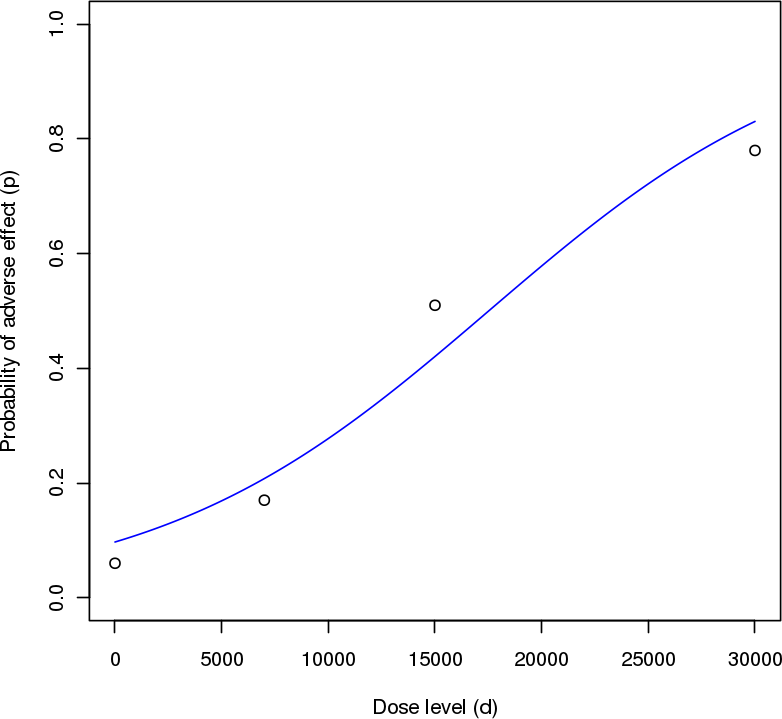
\includegraphics[width=0.48\linewidth]{Images/testA8.png} \quad  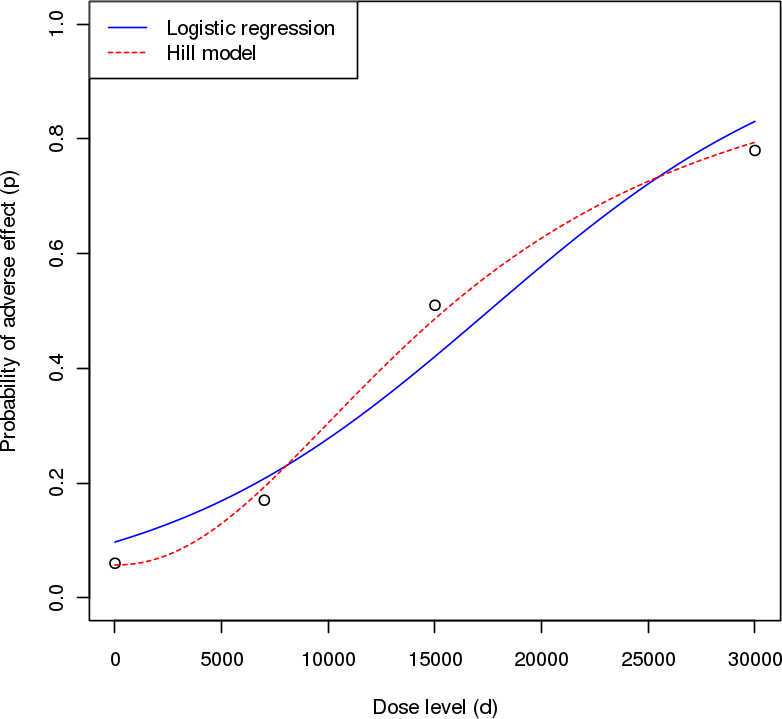
\includegraphics[width=0.48\linewidth]{Images/testA9.png}
  \caption{\small Dose-response model for C.I. Acid Red 114 using logistic regression (blue) and the Hill model (red).}
  \label{fig:testA8}\hrule
\end{figure*}
\subsection{Relationship to Linear Regression}
Since $p_{d}$ is a probability, it has to lie in $[0,1]$. Let the odds of having an adverse effect be $\omega_{d}=p_{d}/(1-p_{d})$; $\omega_d$ now lies in $[0,\infty)$, and the log odds $\ln \omega_d$ will span $\mathbb{R}$. The functional form of the \textbf{logistic regression model} is 
$$
    \log(\omega_{d})=\log\left(\frac{p_{d}}{1-p_{d}}\right)=\beta_{0}+\beta_{1}d,
$$
which is a simple linear regression model.

\subsection{Other Non-Linear Regression Models}
Other \textbf{sigmoidal curves} can be used to model the relationship between predictors and a binary response variable. \newl Popular alternatives include:
\begin{itemize}[noitemsep]
\item the \textbf{probit} link $P(y|x)=\Phi(\beta_{0}+\beta_{1}x)$, where $\Phi$ is the cumulative distribution function of the standard normal distribution, or 
\item the \textbf{complementary log-log} link $$P(y|x)=1-\exp(-\exp(\beta_{0}+\beta_{1}x)).$$ \end{itemize}
In toxicology studies, one of the most widely used model is called the \textbf{Hill}model, and it is defined \textit{via} 
\begin{equation*}
    P(y|d,\alpha, \kappa, \eta)=\alpha + (1-\alpha)\frac{d^{\eta}}{d^{\eta}+\kappa^{\eta}};
\end{equation*}
part of its appeal to health scientists is the interpretation of its parameters -- $\alpha$ represents the \textbf{background rate for adverse effect}, while $\kappa$ denotes $\textrm{ED}_{50}$ (the \textbf{effective dose at which $50\%$ of participants would exhibit the response of interest}) and $\eta$ provides the \textbf{steepness of the dose-response curve}. \newl Figure \ref{fig:testA8} (on the right) compares the simple logistic model to the Hill model; we observe that the Hill model provides a closer fit to the observed proportions, and the curvature is more pronounced compared to the logistic model.




%%%%%%%%%%%%%%%%%%%%%%%%%%%%%%%Section 11%%%%%%%%%%%%%%%%%%%%%%%%%%%%%%%%%%% 

